\documentclass[14pt, a4paper]{article}
\usepackage[T2A]{fontenc}
\usepackage[utf8]{inputenc}
\usepackage[russian]{babel}
\usepackage[left=3cm, right=1.5cm, top=2cm, bottom=2cm]{geometry}
\usepackage{indentfirst}
\usepackage{microtype}
\usepackage{array}
\usepackage{xcolor}
% \usepackage{times}
\usepackage{tempora}
\usepackage{ulem}
\usepackage{setspace}
\usepackage{amsmath}
\usepackage{booktabs}
\usepackage{graphicx}
\usepackage{float}
\usepackage{listings}
\graphicspath{{reports/figures/}{figures/}}
\lstset{basicstyle=\ttfamily\small, breaklines=true, columns=fullflexible, frame=single, keepspaces=true}
\pagestyle{empty}

\makeatletter
\renewcommand\section{\@startsection {section}{1}{\parindent}%
  {-3.5ex \@plus -1ex \@minus -.2ex}%
  {0.5ex}%
  {\normalfont\Large\bfseries}}
\renewcommand\tableofcontents{%
  \begin{center}\Large\bfseries\contentsname\end{center}%
  \@starttoc{toc}%
}
\renewcommand*\l@section{\@dottedtocline{1}{0em}{1.5em}}
\makeatother

\begin{document}
\onehalfspacing

\begin{center}
    \textbf{ФЕДЕРАЛЬНОЕ ГОСУДАРСТВЕННОЕ АВТОНОМНОЕ ОБРАЗОВАТЕЛЬНОЕ} \\
    \textbf{УЧРЕЖДЕНИЕ ВЫСШЕГО ОБРАЗОВАНИЯ} \\
    \textbf{«МОСКОВСКИЙ АВИАЦИОННЫЙ ИНСТИТУТ} \\
    \textbf{(НАЦИОНАЛЬНЫЙ ИССЛЕДОВАТЕЛЬСКИЙ УНИВЕРСИТЕТ)»}
\end{center}

\begin{center}
    \bfseries Институт №8 «Компьютерные науки и \\
    \bfseries прикладная математика» \\
    \bfseries Кафедра 806 «Вычислительная математика \\
    \bfseries и программирование»
\end{center}

\vspace{3cm}

\begin{center}
    \Large\bfseries Отчет \\
    \vspace{0.5cm}
    \mdseries по лабораторной работе №1.1
\end{center}

\vfill

\noindent
\hfill
\begin{tabular}{ll}
Группа:       & М8О-307Б-21 \\
Студент:      & М. С. Ивченко \\
Преподаватель:& доц. В. В. Киндинова \\
Оценка:       & \underline{\makebox[3cm][c]{}} \\ [0.2cm]
Дата:         & \underline{\makebox[3cm][c]{}}
\end{tabular}

\vfill

\begin{center}
    Москва \\
    2026
\end{center}

\newpage

\setcounter{tocdepth}{2}
\tableofcontents
\newpage

\section*{Тема}
\addcontentsline{toc}{section}{Тема}
Цель данной лабораторной работы -- познакомиться с прямыми методами решения систем линейных алгебраических уравнений. В работе рассматривается LU-разложение с выбором главного элемента: этот подход позволяет не только найти решение СЛАУ, но и получить дополнительные характеристики матрицы, такие как определитель и обратная матрица.

\section*{Задание}
\addcontentsline{toc}{section}{Задание}
Реализовать алгоритм $LU$-разложения матриц (с выбором главного элемента) в виде программы. Используя разработанное программное обеспечение, решить систему линейных алгебраических уравнений (СЛАУ). Для матрицы СЛАУ вычислить определитель и обратную матрицу.

\section*{Теория}
\addcontentsline{toc}{section}{Теория}
LU-разложение является прямым методом решения СЛАУ. Его идея состоит в том, чтобы заменить решение исходной системы $Ax=b$ решением двух более простых систем с треугольными матрицами. Для невырожденной матрицы после возможных перестановок строк можно получить представление
\[
    PA = LU,
\]
где $P$ -- матрица перестановок, $L$ -- нижняя треугольная матрица с единичной диагональю, $U$ -- верхняя треугольная матрица. Если перестановки не учитывать, алгоритм может потребовать деления на малый или нулевой ведущий элемент. Поэтому используется частичный выбор главного элемента: на шаге $k$ среди строк $k,\ldots,n$ выбирается строка с максимальным $|a_{ik}|$ в текущем столбце и переносится на диагональную позицию.

Разложение можно рассматривать как компактную запись метода Гаусса. Элементы матрицы $U$ образуются из текущей ведущей строки, а элементы $L$ являются множителями, на которые умножается ведущая строка при исключении неизвестной из нижних строк:
\[
    l_{ik}=\frac{a_{ik}^{(k)}}{u_{kk}}, \qquad
    a_{ij}^{(k+1)}=a_{ij}^{(k)}-l_{ik}u_{kj}, \quad i,j\ge k.
\]
Единицы на диагонали $L$ фиксируют, что множители исключения хранятся только ниже диагонали. Если на некотором шаге после выбора главного элемента $u_{kk}=0$, матрица вырождена и единственного решения может не существовать.

СЛАУ $Ax=b$ после разложения решается двумя треугольными проходами:
\[
    Lz = Pb, \qquad Ux = z.
\]
Сначала прямой подстановкой находится вектор $z$, затем обратной подстановкой находится $x$. Такой подход особенно выгоден, если нужно решать несколько систем с одной и той же матрицей $A$: разложение строится один раз, а затем меняются только правые части.

Определитель равен произведению диагональных элементов $U$ с учетом четности перестановки строк:
\[
    \det A = (-1)^s\prod_i u_{ii}.
\]
Здесь $s$ -- число перестановок строк. Обратная матрица находится решением систем $AX_i=e_i$ для всех столбцов единичной матрицы. Полученные решения $X_i$ записываются в столбцы $A^{-1}$. Корректность результата проверяется по невязке $Ax-b$ и по близости произведения $AA^{-1}$ к единичной матрице.

\begin{lstlisting}[language=Python]
for k in range(n):
    pivot_idx = max(range(k, n), key=lambda i: abs(A_k[i, k]))
    if pivot_idx != k:
        A_k[[pivot_idx, k]] = A_k[[k, pivot_idx]]
        L[[pivot_idx, k]] = L[[k, pivot_idx]]
        p[pivot_idx], p[k] = p[k], p[pivot_idx]
    U[k, k:] = A_k[k, k:]
    L[k:, k] = A_k[k:, k] / U[k, k]
    A_k[k:, k:] -= np.outer(L[k:, k], U[k, k:])
\end{lstlisting}

\section*{Ход лабораторной работы}
\addcontentsline{toc}{section}{Ход лабораторной работы}
Для варианта использовалась система
\[
A=\begin{pmatrix}
2&-8&0&5\\
-9&9&-7&6\\
-6&7&3&8\\
-1&8&5&1
\end{pmatrix},\qquad
b=\begin{pmatrix}-40&-58&-75&1\end{pmatrix}^T.
\]
После выбора главных элементов получен вектор перестановок $p=(1,3,2,0)$. Решение треугольных систем дало
\[
    x=(7,\;3,\;-2,\;-6)^T.
\]
Невязка $b-Ax$ не превышает $9.6\cdot 10^{-7}$ по модулю, что соответствует погрешности машинных вычислений.

\begin{table}[H]
\centering
\begin{tabular}{rrrr}
\toprule
\multicolumn{4}{c}{$A^{-1}$}\\
\midrule
 0.331839& 0.174888&-0.399103& 0.484305\\
 0.092177& 0.104136&-0.166418& 0.245640\\
-0.124066&-0.150972& 0.207773&-0.136024\\
 0.214748& 0.096662&-0.106627& 0.199302\\
\bottomrule
\end{tabular}
\caption{Обратная матрица, найденная через решение систем с единичными правыми частями.}
\end{table}
\[
    \det A = -2007.
\]

\begin{figure}[H]
    \centering
    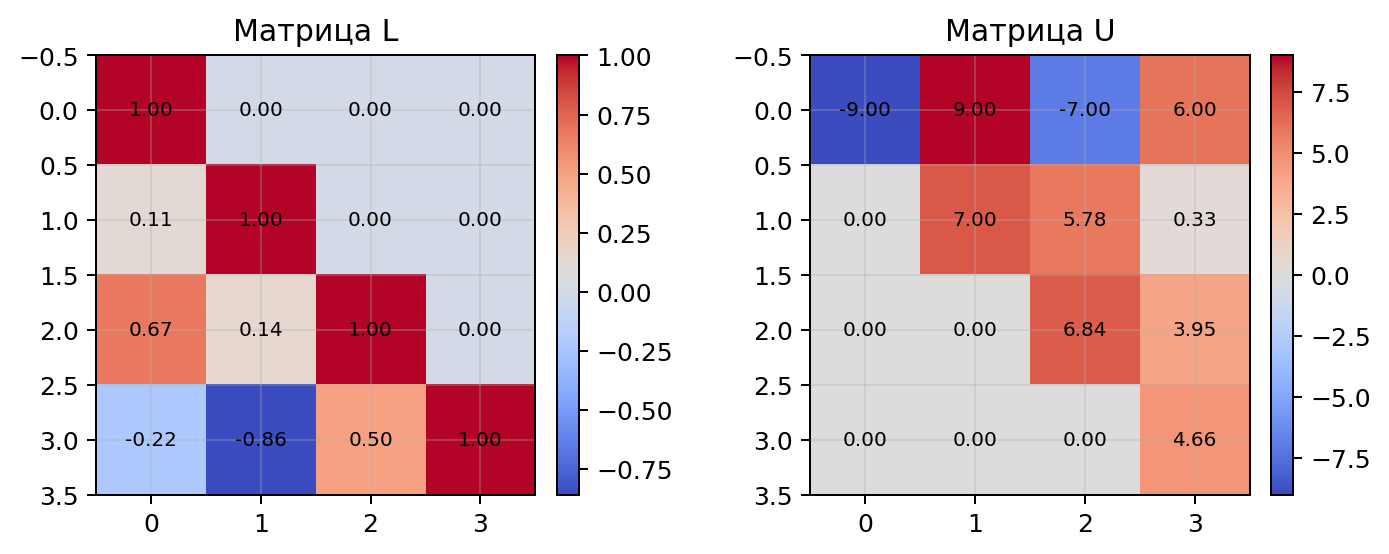
\includegraphics[width=0.86\textwidth]{lab1_1_lu.png}
    \caption{Матрицы $L$ и $U$, полученные при LU-разложении с выбором главного элемента.}
\end{figure}

\section*{Выводы}
\addcontentsline{toc}{section}{Выводы}
LU-разложение с перестановками строк позволило устойчиво решить СЛАУ, вычислить определитель и обратную матрицу в рамках одного разложения. Проверки $LU=PA$, $Ax\approx b$ и $AA^{-1}\approx I$ показали только ошибки порядка машинного округления.

\end{document}
